\section{INLA for Gaussian Data}

- It is a latent gausian model, these are a subclass of the structured additive regression models - > y belongs to the exponential family. In addition all latent variabler have gausian priors. 

%Dette er structured additiv model
\begin{equation}
\begin{split}
    g(\mu_i) = \eta_i = \alpha + \sum_{k = 1}^{n_\beta} \beta_k z_{mi} + \sum_{j = 1}^{n_f}f^{(j)}(u_{ji}) + \epsilon_i
\end{split}
\end{equation}

- i tillegg må the latent field være cond indep, i vårt tilfelle være $\eta_i$ ene
- siste punkt er få hyperparametere

\subsection{Plotting the data}
 
\begin{figure}
    \centering
    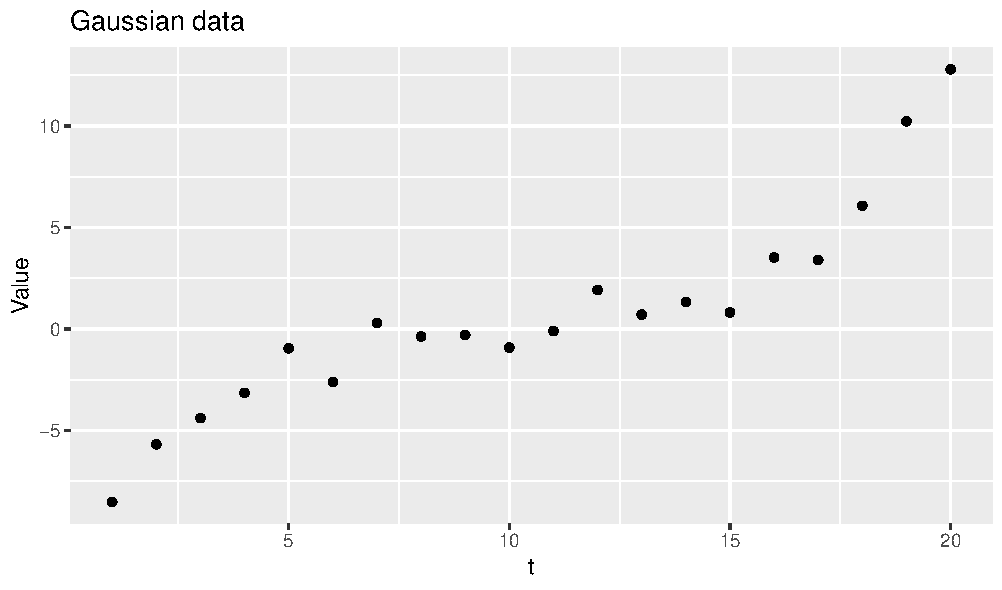
\includegraphics[width=\textwidth]{Images/gaussian_data.pdf}
    \caption{Caption}
    \label{fig:gaussian_data}
\end{figure}

- skriv in hva pressicion matrixen Q blir

\subsection{Latent Gaussian model, and the possibility of using INLA to estimate the parameters in the model}

\subsection{Implementing a block Gibbs sampling algorithm for $f(\eta, \theta |y)$}

- skriv inn the full conditional for $\pi(\theta|\eta, y)$ og $\pi(\eta|\theta, y)$

\subsubsection{Proposing a new value for $\theta$ from the full conditional $\pi(\theta | \eta,y)$}

\subsubsection{Proposing a new value for the $\eta$-vector from the full conditional $\pi(\eta | \theta, y)$}

\subsection{Estimate for the posterior marginal for the hyperparameter $\pi(\theta|y)$}

\subsubsection{Estimate of the smooth effect using the mean and pointwise a $95 \%$ confidence bound around the mean}

\subsection{Approximating the posterior marginal for the hyperparameter $\theta$, $\pi(\theta|y)$ using the INLA scheme}

\subsubsection{Approximation for $\pi(\theta|y)$}

\subsection{Implementing the approximation of the marginal posterior for the smooth effect, $\pi(\eta_i | y)$}

\subsection{Using the inla() - function in R to implement the model,and comparing the results}

